%%%%%%%%%%%%%%%%%%%%%%%%%%%%%%%%%%%%%%%
% Wenneker Resume/CV
% LaTeX Template
% Version 1.1 (19/6/2016)
%
% This template has been downloaded from:
% http://www.LaTeXTemplates.com
%
% Original author:
% Frits Wenneker (http://www.howtotex.com) with extensive modifications by 
% Vel (vel@LaTeXTemplates.com)
%
% License:
% CC BY-NC-SA 3.0 (http://creativecommons.org/licenses/by-nc-sa/3.0/
%
%%%%%%%%%%%%%%%%%%%%%%%%%%%%%%%%%%%%%%

%----------------------------------------------------------------------------------------
%	PACKAGES AND OTHER DOCUMENT CONFIGURATIONS
%----------------------------------------------------------------------------------------

\documentclass[a4paper,12pt]{memoir} % Font and paper size

%%%%%%%%%%%%%%%%%%%%%%%%%%%%%%%%%%%%%%%%%
% Wenneker Resume/CV
% Structure Specification File
% Version 1.1 (19/6/2016)
%
% This file has been downloaded from:
% http://www.LaTeXTemplates.com
%
% Original author:
% Frits Wenneker (http://www.howtotex.com) with extensive modifications by 
% Vel (vel@latextemplates.com)
%
% License:
% CC BY-NC-SA 3.0 (http://creativecommons.org/licenses/by-nc-sa/3.0/)
%
%%%%%%%%%%%%%%%%%%%%%%%%%%%%%%%%%%%%%%%%%

%----------------------------------------------------------------------------------------
%	PACKAGES AND OTHER DOCUMENT CONFIGURATIONS
%----------------------------------------------------------------------------------------

\usepackage{XCharter} % Use the Bitstream Charter font
\usepackage[utf8]{inputenc} % Required for inputting international characters
\usepackage[T1]{fontenc} % Output font encoding for international characters

\usepackage[top=1cm,left=1cm,right=1cm,bottom=1cm]{geometry} % Modify margins

\usepackage{graphicx} % Required for figures

\usepackage{flowfram} % Required for the multi-column layout

\usepackage{url} % URLs

\usepackage[usenames,dvipsnames]{xcolor} % Required for custom colours

\usepackage{tikz} % Required for the horizontal rule

\usepackage{enumitem} % Required for modifying lists
\setlist{noitemsep,nolistsep} % Remove spacing within and around lists

\setlength{\columnsep}{\baselineskip} % Set the spacing between columns

% Define the left frame (sidebar)
\newflowframe{0.2\textwidth}{\textheight}{0pt}{0pt}[left]
\newlength{\LeftMainSep}
\setlength{\LeftMainSep}{0.2\textwidth}
\addtolength{\LeftMainSep}{1\columnsep}
 
% Small static frame for the vertical line
\newstaticframe{1.5pt}{\textheight}{\LeftMainSep}{0pt}
 
% Content of the static frame with the vertical line
\begin{staticcontents}{1}
\hfill
\tikz{\draw[loosely dotted,color=RoyalBlue,line width=1.5pt,yshift=0](0,0) -- (0,\textheight);}
\hfill\mbox{}
\end{staticcontents}
 
% Define the right frame (main body)
\addtolength{\LeftMainSep}{1.5pt}
\addtolength{\LeftMainSep}{1\columnsep}
\newflowframe{0.7\textwidth}{\textheight}{\LeftMainSep}{0pt}[main01]

\pagestyle{empty} % Disable all page numbering

\setlength{\parindent}{0pt} % Stop paragraph indentation

%----------------------------------------------------------------------------------------
%	NEW COMMANDS
%----------------------------------------------------------------------------------------

\newcommand{\userinformation}[1]{\renewcommand{\userinformation}{#1}} % Define a new command for the CV user's information that goes into the left column

\newcommand{\cvheading}[1]{{\Huge\bfseries\color{RoyalBlue} #1} \par\vspace{.6\baselineskip}} % New command for the CV heading
\newcommand{\cvsubheading}[1]{{\Large\bfseries #1} \bigbreak} % New command for the CV subheading

\newcommand{\Sep}{\vspace{1em}} % New command for the spacing between headings
\newcommand{\SmallSep}{\vspace{0.5em}} % New command for the spacing within headings

\newcommand{\aboutme}[2]{ % New command for the about me section
\textbf{\color{RoyalBlue} #1}~~#2\par\Sep
}
	
\newcommand{\CVSection}[1]{ % New command for the headings within sections
{\Large\textbf{#1}}\par
\SmallSep % Used for spacing
}

\newcommand{\CVItem}[2]{ % New command for the item descriptions
\textbf{\color{RoyalBlue} #1}\par
#2
\SmallSep % Used for spacing
}

\newcommand{\bluebullet}{\textcolor{RoyalBlue}{$\circ$}~~} % New command for the blue bullets
 % Include the file specifying document layout and packages

%----------------------------------------------------------------------------------------
%	NAME AND CONTACT INFORMATION 
%----------------------------------------------------------------------------------------

\userinformation{ % Set the content that goes into the sidebar of each page
\begin{flushright}
% Comment out this figure block if you don't want a photo
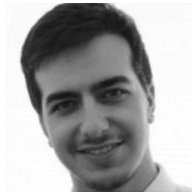
\includegraphics[width=0.6\columnwidth]{photo.jpg}\\[\baselineskip] % Your photo
\small % Smaller font size
André Pascoal Bento \\ % Your name
\url{apbento@student.dei.uc.pt} \\ % Your email address
%\url{abento.site} \\ % Your URL
(+351)~910~349~466 \\ % Your phone number
(+351)~231~488~174 \\ % My fixed number 
\Sep % Some whitespace
\textbf{Address} \\
R. Dr. António \\ José de Almeida, n.98 \\ % Address 1
Mira, 3070-399 \\ % Address 2
Coimbra, Portugal \\ % Address 3
\vfill % Whitespace under this block to push it up under the photo
\end{flushright}
}

%----------------------------------------------------------------------------------------

\begin{document}

\userinformation % Print your information in the left column

\framebreak % End of the first column

%----------------------------------------------------------------------------------------
%	HEADING
%----------------------------------------------------------------------------------------

\cvheading{André Bento} % Large heading - your name

\cvsubheading{PhD Student @ University of Coimbra} % \\ Informatics Engineering} % Subheading - your occupation/specialization

%----------------------------------------------------------------------------------------
%	ABOUT ME
%----------------------------------------------------------------------------------------

\aboutme{About Me}{I am a person who loves knowledge sharing, inter-help, technology, and meeting new people. Energetic and advocate about software development with the objective of beign on top of new trends in the area.}

%----------------------------------------------------------------------------------------
%	EDUCATION
%----------------------------------------------------------------------------------------

\CVSection{Education}

%------------------------------------------------

\CVItem{2019 - Present, University of Coimbra}{PhD in Information Science and Technology}

%------------------------------------------------

\CVItem{2017 - 2019, University of Coimbra}{MSc in Informatics Engineering}

%------------------------------------------------

\CVItem{2014 - 2017, Coimbra Institute of Engineering (ISEC)}{BSc in Informatics Engineering}

%------------------------------------------------

\Sep % Extra whitespace after the end of a major section

%----------------------------------------------------------------------------------------
%	EXPERIENCE
%----------------------------------------------------------------------------------------

\CVSection{Experience}

%------------------------------------------------

\CVItem{Feb 2017 - Jul 2017, \textit{Software Engineer Internship}, \\WIT Software, S.A.}{
%Detailed achievements:
\begin{itemize}
	\item Android app development:
	\begin{itemize}
		\item Selfies and enhanced user content creation
		\item Digital filters and image manipulation (Stickers, colour filters, handwriting and drawing)
		\begin{itemize}
			\item Java for Android native development
			\item Canvas and OpenGL
			%\item MVVM design pattern
		\end{itemize}
	\end{itemize}
	\item Integrated a multidisciplinary software development team 
	\item Participated in Android, iOS, Git, Programming languages and Project Management talk workshops 
	\item Team building activities and vacations  
	\item Drank many coffees with pleasant fellows
\end{itemize}
}

%------------------------------------------------

\CVItem{Nov 2016 - Jun 2017, \textit{Scratch Programming Teacher}, CASPAE - IPSS}{
%Detailed achievements:
\begin{itemize}
	\item Teaching primary school students scratch programming language and problem solving
	%\item Teaching primary school students:
	%\begin{itemize}
	%	\item Scratch programming language
	%	\item Problem solving
	%\end{itemize}
	%\item Contact with teaching fourth grade students
	%\item Volunteered worker
\end{itemize}
}

%------------------------------------------------

\CVItem{Nov 2015 - Mar 2016, \textit{Math Applied to Engineer Teacher}, CeAMatE}{
%Detailed achievements:
\begin{itemize}
	\item Teaching pre-degree, CTeSP and Engineering students %important concepts of mathematics
	\item Helped preparing them for:
	\begin{itemize}
		\item High-School and University final math exams
	\end{itemize}
\end{itemize}
}

%------------------------------------------------

%\CVItem{Feb 2017 - Jul 2017, \textit{Accountant Technician Internship}, \\Caixa de Crédito Agrícola Mútuo de Cantanhede e Mira - C.R.L.}{
%Detailed achievements:
%\begin{itemize}
%	\item bank accountment,
%bank organization and bank day-to-day work
%	\item Drank many coffees with pleasant fellows
%\end{itemize}
%}


%\CVItem{Nov 2008 - Oct 2012, \textit{Computer Repair Specialist}, Buy More}{Worked in the Nerd Herd and helped to solve computer problems by asking customers to turn their computers off and on again.}

%------------------------------------------------

\Sep % Extra whitespace after the end of a major section

%----------------------------------------------------------------------------------------
%	COMMUNICATION SKILLS
%----------------------------------------------------------------------------------------

\CVSection{Communication Skills}

%------------------------------------------------

{\begin{tabular}{p{0.3\textwidth} p{0.3\textwidth}}
\bluebullet Portuguese (native) &  \bluebullet English (advanced) \\
\bluebullet Spanish (intermediate) %& \bluebullet Deutsch (beginner) \\
%& \bluebullet French (beginner)
\end{tabular}}

%\CVItem{2015, \textit{Oral Presentation}, California Business Conference}{Presented research I conducted for my Masters of Engineering degree.}

%------------------------------------------------

%\CVItem{2014, \textit{Poster}, Annual Business Conference (Oregon)}{As part of the course work for BUS320, I created a poster analyzing several local businesses and presented this at a conference.}

%------------------------------------------------

%\Sep % Extra whitespace after the end of a major section

%----------------------------------------------------------------------------------------
%	SKILLS
%----------------------------------------------------------------------------------------

%\CVSection{Software Development Skills}

%------------------------------------------------

%\CVItem{Programming}
%{\begin{tabular}{p{0.2\textwidth} p{0.2\textwidth} p{0.2\textwidth}}
%\bluebullet Java &  \bluebullet Shell & \bluebullet Python\\
%\bluebullet C++ &  \bluebullet PHP & \bluebullet Matlab\\
%\end{tabular}}

%------------------------------------------------

%\CVItem{Computer Software}
%{\begin{tabular}{p{0.2\textwidth} p{0.2\textwidth} p{0.2\textwidth}}
% \bluebullet MySQL &  \bluebullet iOS & \bluebullet Android\\
%\end{tabular}}

%------------------------------------------------

%\Sep % Extra whitespace after the end of a major section

%----------------------------------------------------------------------------------------
%	NEW PAGE DELIMITER
%	Place this block wherever you would like the content of your CV to go onto the next page
%----------------------------------------------------------------------------------------

%\clearpage % Start a new page

%\userinformation % Print your information in the left column

%\framebreak % End of the first column

%----------------------------------------------------------------------------------------
%	AWARDS
%----------------------------------------------------------------------------------------

%\CVSection{Awards}

%------------------------------------------------

%\CVItem{2010, \textit{Postgraduate Scholarship}, Cornell University}{Awarded to the top student in their final year of a Bachelors degree.}

%------------------------------------------------

\Sep % Extra whitespace after the end of a major section

%----------------------------------------------------------------------------------------
%	INTERESTS
%----------------------------------------------------------------------------------------

\CVSection{Interests}

%------------------------------------------------

\CVItem{Professional}{Microservices, Cloud computing, Tracing, Monitoring, Data analysis, \\Machine learning, Programming languages and Software development}

%------------------------------------------------

\CVItem{Personal}{Traveling, Swimming, Treking, Long walks, Kayak and Canoeing \\Having fun with family and friends}

%------------------------------------------------

\Sep % Extra whitespace after the end of a major section

%----------------------------------------------------------------------------------------

\end{document}
